\documentclass[]{article}
\usepackage{lmodern}
\usepackage{amssymb,amsmath}
\usepackage{ifxetex,ifluatex}
\usepackage{fixltx2e} % provides \textsubscript
\ifnum 0\ifxetex 1\fi\ifluatex 1\fi=0 % if pdftex
  \usepackage[T1]{fontenc}
  \usepackage[utf8]{inputenc}
\else % if luatex or xelatex
  \ifxetex
    \usepackage{mathspec}
  \else
    \usepackage{fontspec}
  \fi
  \defaultfontfeatures{Ligatures=TeX,Scale=MatchLowercase}
\fi
% use upquote if available, for straight quotes in verbatim environments
\IfFileExists{upquote.sty}{\usepackage{upquote}}{}
% use microtype if available
\IfFileExists{microtype.sty}{%
\usepackage{microtype}
\UseMicrotypeSet[protrusion]{basicmath} % disable protrusion for tt fonts
}{}
\usepackage[margin=1in]{geometry}
\usepackage{hyperref}
\hypersetup{unicode=true,
            pdftitle={mTSC Food Intake Analysis},
            pdfauthor={Dave Bridges, Molly C. Mulcahy, and Detrick Snyder},
            pdfborder={0 0 0},
            breaklinks=true}
\urlstyle{same}  % don't use monospace font for urls
\usepackage{color}
\usepackage{fancyvrb}
\newcommand{\VerbBar}{|}
\newcommand{\VERB}{\Verb[commandchars=\\\{\}]}
\DefineVerbatimEnvironment{Highlighting}{Verbatim}{commandchars=\\\{\}}
% Add ',fontsize=\small' for more characters per line
\usepackage{framed}
\definecolor{shadecolor}{RGB}{248,248,248}
\newenvironment{Shaded}{\begin{snugshade}}{\end{snugshade}}
\newcommand{\KeywordTok}[1]{\textcolor[rgb]{0.13,0.29,0.53}{\textbf{#1}}}
\newcommand{\DataTypeTok}[1]{\textcolor[rgb]{0.13,0.29,0.53}{#1}}
\newcommand{\DecValTok}[1]{\textcolor[rgb]{0.00,0.00,0.81}{#1}}
\newcommand{\BaseNTok}[1]{\textcolor[rgb]{0.00,0.00,0.81}{#1}}
\newcommand{\FloatTok}[1]{\textcolor[rgb]{0.00,0.00,0.81}{#1}}
\newcommand{\ConstantTok}[1]{\textcolor[rgb]{0.00,0.00,0.00}{#1}}
\newcommand{\CharTok}[1]{\textcolor[rgb]{0.31,0.60,0.02}{#1}}
\newcommand{\SpecialCharTok}[1]{\textcolor[rgb]{0.00,0.00,0.00}{#1}}
\newcommand{\StringTok}[1]{\textcolor[rgb]{0.31,0.60,0.02}{#1}}
\newcommand{\VerbatimStringTok}[1]{\textcolor[rgb]{0.31,0.60,0.02}{#1}}
\newcommand{\SpecialStringTok}[1]{\textcolor[rgb]{0.31,0.60,0.02}{#1}}
\newcommand{\ImportTok}[1]{#1}
\newcommand{\CommentTok}[1]{\textcolor[rgb]{0.56,0.35,0.01}{\textit{#1}}}
\newcommand{\DocumentationTok}[1]{\textcolor[rgb]{0.56,0.35,0.01}{\textbf{\textit{#1}}}}
\newcommand{\AnnotationTok}[1]{\textcolor[rgb]{0.56,0.35,0.01}{\textbf{\textit{#1}}}}
\newcommand{\CommentVarTok}[1]{\textcolor[rgb]{0.56,0.35,0.01}{\textbf{\textit{#1}}}}
\newcommand{\OtherTok}[1]{\textcolor[rgb]{0.56,0.35,0.01}{#1}}
\newcommand{\FunctionTok}[1]{\textcolor[rgb]{0.00,0.00,0.00}{#1}}
\newcommand{\VariableTok}[1]{\textcolor[rgb]{0.00,0.00,0.00}{#1}}
\newcommand{\ControlFlowTok}[1]{\textcolor[rgb]{0.13,0.29,0.53}{\textbf{#1}}}
\newcommand{\OperatorTok}[1]{\textcolor[rgb]{0.81,0.36,0.00}{\textbf{#1}}}
\newcommand{\BuiltInTok}[1]{#1}
\newcommand{\ExtensionTok}[1]{#1}
\newcommand{\PreprocessorTok}[1]{\textcolor[rgb]{0.56,0.35,0.01}{\textit{#1}}}
\newcommand{\AttributeTok}[1]{\textcolor[rgb]{0.77,0.63,0.00}{#1}}
\newcommand{\RegionMarkerTok}[1]{#1}
\newcommand{\InformationTok}[1]{\textcolor[rgb]{0.56,0.35,0.01}{\textbf{\textit{#1}}}}
\newcommand{\WarningTok}[1]{\textcolor[rgb]{0.56,0.35,0.01}{\textbf{\textit{#1}}}}
\newcommand{\AlertTok}[1]{\textcolor[rgb]{0.94,0.16,0.16}{#1}}
\newcommand{\ErrorTok}[1]{\textcolor[rgb]{0.64,0.00,0.00}{\textbf{#1}}}
\newcommand{\NormalTok}[1]{#1}
\usepackage{longtable,booktabs}
\usepackage{graphicx,grffile}
\makeatletter
\def\maxwidth{\ifdim\Gin@nat@width>\linewidth\linewidth\else\Gin@nat@width\fi}
\def\maxheight{\ifdim\Gin@nat@height>\textheight\textheight\else\Gin@nat@height\fi}
\makeatother
% Scale images if necessary, so that they will not overflow the page
% margins by default, and it is still possible to overwrite the defaults
% using explicit options in \includegraphics[width, height, ...]{}
\setkeys{Gin}{width=\maxwidth,height=\maxheight,keepaspectratio}
\IfFileExists{parskip.sty}{%
\usepackage{parskip}
}{% else
\setlength{\parindent}{0pt}
\setlength{\parskip}{6pt plus 2pt minus 1pt}
}
\setlength{\emergencystretch}{3em}  % prevent overfull lines
\providecommand{\tightlist}{%
  \setlength{\itemsep}{0pt}\setlength{\parskip}{0pt}}
\setcounter{secnumdepth}{5}
% Redefines (sub)paragraphs to behave more like sections
\ifx\paragraph\undefined\else
\let\oldparagraph\paragraph
\renewcommand{\paragraph}[1]{\oldparagraph{#1}\mbox{}}
\fi
\ifx\subparagraph\undefined\else
\let\oldsubparagraph\subparagraph
\renewcommand{\subparagraph}[1]{\oldsubparagraph{#1}\mbox{}}
\fi

%%% Use protect on footnotes to avoid problems with footnotes in titles
\let\rmarkdownfootnote\footnote%
\def\footnote{\protect\rmarkdownfootnote}

%%% Change title format to be more compact
\usepackage{titling}

% Create subtitle command for use in maketitle
\newcommand{\subtitle}[1]{
  \posttitle{
    \begin{center}\large#1\end{center}
    }
}

\setlength{\droptitle}{-2em}

  \title{mTSC Food Intake Analysis}
    \pretitle{\vspace{\droptitle}\centering\huge}
  \posttitle{\par}
    \author{Dave Bridges, Molly C. Mulcahy, and Detrick Snyder}
    \preauthor{\centering\large\emph}
  \postauthor{\par}
      \predate{\centering\large\emph}
  \postdate{\par}
    \date{October 2019}


\begin{document}
\maketitle

{
\setcounter{tocdepth}{2}
\tableofcontents
}
\section{Raw Data}\label{raw-data}

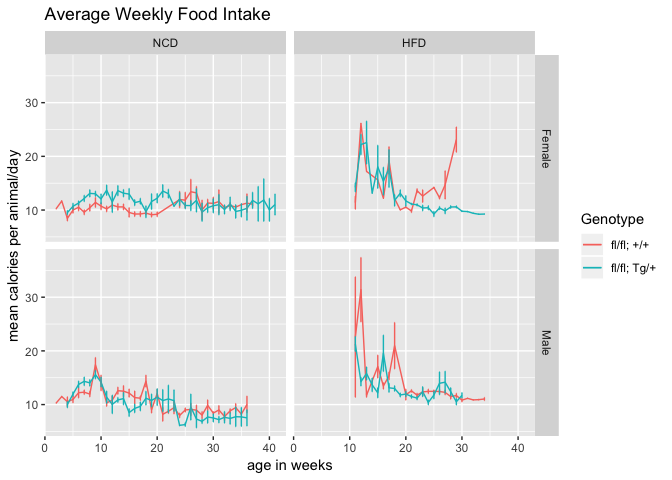
\includegraphics{figures/intake-graphs-1.png} These data can be found in
\textbf{/Users/davebrid/Documents/GitHub/TissueSpecificTscKnockouts/Mouse
Data/Muscle Tsc1 Knockout} in a file named \textbf{Food Intake Log.csv}.
This script was most recently updated on \textbf{Wed Apr 3 15:25:20
2019}. \# Analysis

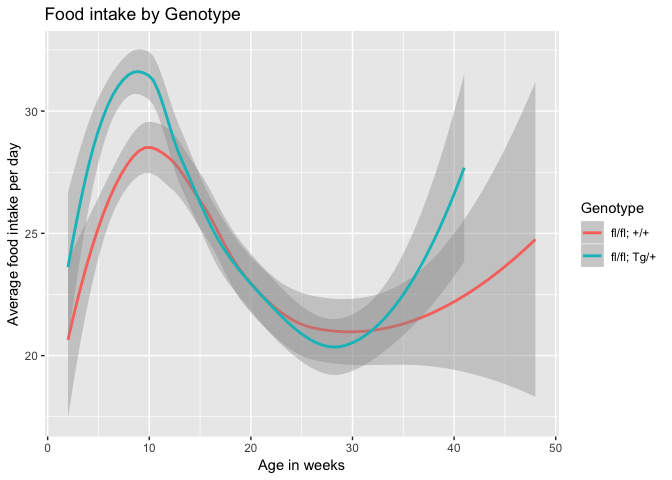
\includegraphics{figures/weekly-intake-plots-1.png}
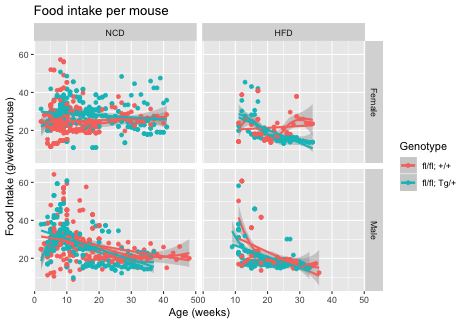
\includegraphics{figures/weekly-intake-plots-2.png}
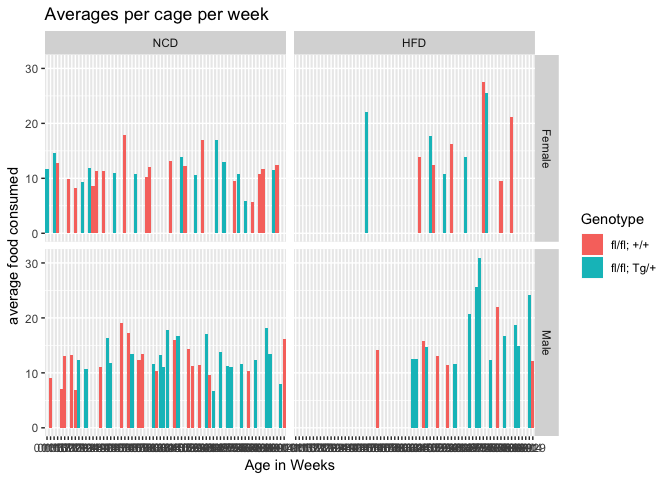
\includegraphics{figures/weekly-intake-plots-3.png}
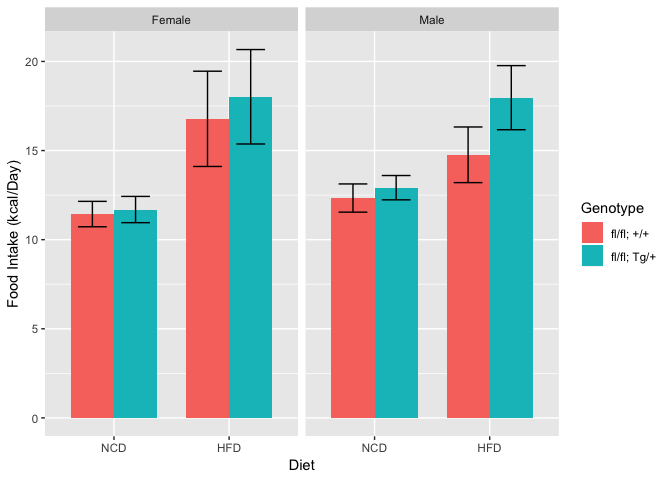
\includegraphics{figures/weekly-intake-plots-4.png}

\begin{verbatim}
##             Df Sum Sq Mean Sq F value Pr(>F)   
## Sex          1    0.0     0.0    0.00 0.9863   
## HFD          1   45.8    45.8   38.02 0.0035 **
## Genotype     1    3.5     3.5    2.89 0.1644   
## Residuals    4    4.8     1.2                  
## ---
## Signif. codes:  0 '***' 0.001 '**' 0.01 '*' 0.05 '.' 0.1 ' ' 1
\end{verbatim}

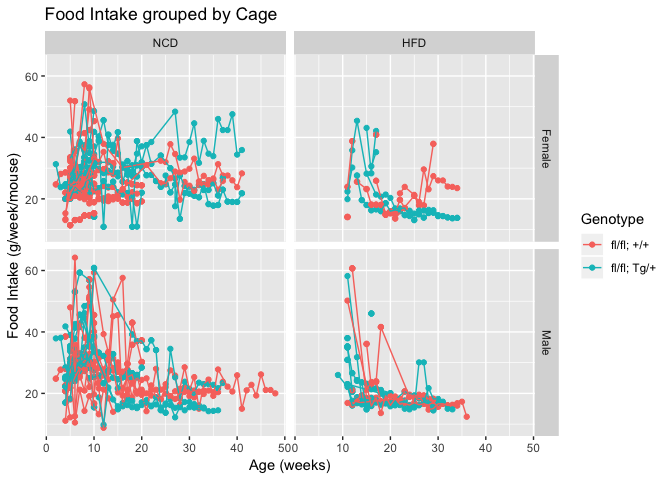
\includegraphics{figures/weekly-lineplot-food-intake-by-cage-1.png}

\subsection{Statistics}\label{statistics}

\begin{verbatim}
## Data: exp.data.22
## Models:
## intake.null: calorie.intake ~ 1 + (1 | Cage)
## intake.lme.hfd: calorie.intake ~ HFD + (1 | Cage)
##                Df  AIC  BIC logLik deviance Chisq Chi Df Pr(>Chisq)    
## intake.null     3 8611 8628  -4303     8605                            
## intake.lme.hfd  4 8542 8563  -4267     8534  71.8      1     <2e-16 ***
## ---
## Signif. codes:  0 '***' 0.001 '**' 0.01 '*' 0.05 '.' 0.1 ' ' 1
\end{verbatim}

\begin{verbatim}
## Data: exp.data.22
## Models:
## intake.lme.hfd: calorie.intake ~ HFD + (1 | Cage)
## intake.lme.age: calorie.intake ~ HFD + age + (1 | Cage)
##                Df  AIC  BIC logLik deviance Chisq Chi Df Pr(>Chisq)    
## intake.lme.hfd  4 8542 8563  -4267     8534                            
## intake.lme.age  5 8397 8424  -4194     8387   146      1     <2e-16 ***
## ---
## Signif. codes:  0 '***' 0.001 '**' 0.01 '*' 0.05 '.' 0.1 ' ' 1
\end{verbatim}

\begin{verbatim}
## Data: exp.data.22
## Models:
## intake.lme.age: calorie.intake ~ HFD + age + (1 | Cage)
## intake.lme.sex: calorie.intake ~ HFD + age + Sex + (1 | Cage)
##                Df  AIC  BIC logLik deviance Chisq Chi Df Pr(>Chisq)
## intake.lme.age  5 8397 8424  -4194     8387                        
## intake.lme.sex  6 8399 8431  -4194     8387  0.14      1       0.71
\end{verbatim}

\begin{longtable}[]{@{}lrrrrrrrr@{}}
\toprule
& Df & AIC & BIC & logLik & deviance & Chisq & Chi Df &
Pr(\textgreater{}Chisq)\tabularnewline
\midrule
\endhead
intake.lme.sex & 6 & 8399 & 8431 & -4194 & 8387 & NA & NA &
NA\tabularnewline
intake.lme.geno & 7 & 8400 & 8438 & -4193 & 8386 & 0.678 & 1 &
0.41\tabularnewline
\bottomrule
\end{longtable}

\begin{longtable}[]{@{}lrrrrrr@{}}
\toprule
& Sum Sq & Mean Sq & NumDF & DenDF & F value &
Pr(\textgreater{}F)\tabularnewline
\midrule
\endhead
HFD & 2033.65 & 2033.65 & 1 & 1361.7 & 174.135 & 0.000\tabularnewline
age & 1788.31 & 1788.31 & 1 & 1488.6 & 153.127 & 0.000\tabularnewline
Sex & 0.88 & 0.88 & 1 & 67.0 & 0.075 & 0.785\tabularnewline
Genotype & 7.49 & 7.49 & 1 & 59.3 & 0.642 & 0.426\tabularnewline
\bottomrule
\end{longtable}

\begin{longtable}[]{@{}lr@{}}
\caption{Pairwise contrasts from mixed linear model, for females on NCD.
The random effect is the cage.}\tabularnewline
\toprule
& x\tabularnewline
\midrule
\endfirsthead
\toprule
& x\tabularnewline
\midrule
\endhead
(Intercept) & 13.319\tabularnewline
HFDHFD & 4.451\tabularnewline
age & -0.166\tabularnewline
SexMale & 0.163\tabularnewline
Genotypefl/fl; Tg/+ & 0.487\tabularnewline
\bottomrule
\end{longtable}

\begin{longtable}[]{@{}llrrrrr@{}}
\toprule
term & levels & Estimate & Std. Error & df & t value &
Pr(\textgreater{}\textbar{}t\textbar{})\tabularnewline
\midrule
\endhead
HFD & NCD - HFD & -4.451 & 0.337 & 1361.7 & -13.196 &
0.000\tabularnewline
Sex & Female - Male & -0.163 & 0.594 & 67.0 & -0.274 &
0.785\tabularnewline
Genotype & fl/fl; +/+ - fl/fl; Tg/+ & -0.487 & 0.608 & 59.3 & -0.801 &
0.426\tabularnewline
\bottomrule
\end{longtable}

\begin{longtable}[]{@{}lllr@{}}
\toprule
Sex & HFD & Genotype & n\tabularnewline
\midrule
\endhead
Female & NCD & fl/fl; +/+ & 17\tabularnewline
Female & NCD & fl/fl; Tg/+ & 13\tabularnewline
Female & HFD & fl/fl; +/+ & 5\tabularnewline
Female & HFD & fl/fl; Tg/+ & 5\tabularnewline
Male & NCD & fl/fl; +/+ & 18\tabularnewline
Male & NCD & fl/fl; Tg/+ & 20\tabularnewline
Male & HFD & fl/fl; +/+ & 6\tabularnewline
Male & HFD & fl/fl; Tg/+ & 12\tabularnewline
\bottomrule
\end{longtable}

\section{Session Information}\label{session-information}

\begin{Shaded}
\begin{Highlighting}[]
\KeywordTok{sessionInfo}\NormalTok{()}
\end{Highlighting}
\end{Shaded}

\begin{verbatim}
## R version 3.5.0 (2018-04-23)
## Platform: x86_64-apple-darwin15.6.0 (64-bit)
## Running under: macOS  10.14.2
## 
## Matrix products: default
## BLAS: /Library/Frameworks/R.framework/Versions/3.5/Resources/lib/libRblas.0.dylib
## LAPACK: /Library/Frameworks/R.framework/Versions/3.5/Resources/lib/libRlapack.dylib
## 
## locale:
## [1] en_US.UTF-8/en_US.UTF-8/en_US.UTF-8/C/en_US.UTF-8/en_US.UTF-8
## 
## attached base packages:
## [1] stats     graphics  grDevices utils     datasets  methods   base     
## 
## other attached packages:
##  [1] broom_0.5.1    lmerTest_3.0-1 lme4_1.1-19    Matrix_1.2-15 
##  [5] dbplyr_1.3.0   car_3.0-2      carData_3.0-2  nlme_3.1-137  
##  [9] ggplot2_3.1.0  bindrcpp_0.2.2 forcats_0.3.0  readr_1.3.1   
## [13] dplyr_0.7.8    tidyr_0.8.2    knitr_1.21    
## 
## loaded via a namespace (and not attached):
##  [1] tidyselect_0.2.5  xfun_0.4          purrr_0.2.5      
##  [4] reshape2_1.4.3    splines_3.5.0     haven_2.0.0      
##  [7] lattice_0.20-38   generics_0.0.2    colorspace_1.3-2 
## [10] htmltools_0.3.6   yaml_2.2.0        rlang_0.3.1      
## [13] nloptr_1.2.1      pillar_1.3.1      foreign_0.8-71   
## [16] glue_1.3.0        withr_2.1.2       DBI_1.0.0        
## [19] readxl_1.2.0      bindr_0.1.1       plyr_1.8.4       
## [22] stringr_1.3.1     munsell_0.5.0     gtable_0.2.0     
## [25] cellranger_1.1.0  zip_1.0.0         evaluate_0.12    
## [28] labeling_0.3      rio_0.5.16        curl_3.2         
## [31] highr_0.7         Rcpp_1.0.0        backports_1.1.3  
## [34] scales_1.0.0      abind_1.4-5       hms_0.4.2        
## [37] digest_0.6.18     stringi_1.2.4     openxlsx_4.1.0   
## [40] numDeriv_2016.8-1 grid_3.5.0        tools_3.5.0      
## [43] magrittr_1.5      lazyeval_0.2.1    tibble_2.0.0     
## [46] crayon_1.3.4      pkgconfig_2.0.2   MASS_7.3-51.1    
## [49] data.table_1.11.8 minqa_1.2.4       assertthat_0.2.0 
## [52] rmarkdown_1.11    R6_2.3.0          compiler_3.5.0
\end{verbatim}


\end{document}
